\chapter{Introducción}
\section{Motivación}
 \begin{itemize}
  \item La seguridad en dispositivos móviles se ha convertido en un asunto muy importante debido al incremento de ataques recibidos y a las consecuencias que éstos tienen.
  \item Los ataques están incentivados por la popularización de los dispositivos móviles, el aumento de información personal y confidencial que almacenan y las operaciones realizadas a través de ellos, como por ejemplo las bancarias.
  \item Actualmente, más del 99\% de los dispositivos móviles en el mercado tiene a iOS o Android como su sistema operativo. El número actual de aplicaciones de Android en el mercado supera los 3.500.00 y para iOS asciende a más de 3.100.000.
  \item Además, debido al uso diario de estas aplicaciones, se puede filtrar una gran cantidad de información privada y confidencial a menos que se aplique control de acceso a las aplicaciones instaladas.
 \end{itemize}
 \begin{paragraph}{Motivación I}
Este trabajo realiza un análisis detallado sobre las características de seguridad en Android e iOS, con el objetivo de preservar la privacidad del usuario.
  \end{paragraph}
  \begin{paragraph}{Motivación II}
Sumado al análisis, se presenta un \emph{framework} comparativo, cuyas principales funciones son:
    \begin{itemize}
     \item Determinar empíricamente los alcances de los sistemas de permisos.
     \item Establecer una relación entre los permisos presenten en ambas plataformas.
    \end{itemize}
   \end{paragraph}
%\subsection{Modelo de Android}
\begin{frame}
 \begin{center}
  \LARGE Modelo de Android
 \end{center}
\end{frame}
\begin{frame}
 \frametitle{Modelo de Android}
 {Android es un sistema operativo de código abierto, diseñado para dispositivos móviles y desarrollado por Google junto con la Open Handset Alliance.}\pause
 \begin{figure}[H]
    \centering
    \begin{subfigure}{0.75\linewidth}
		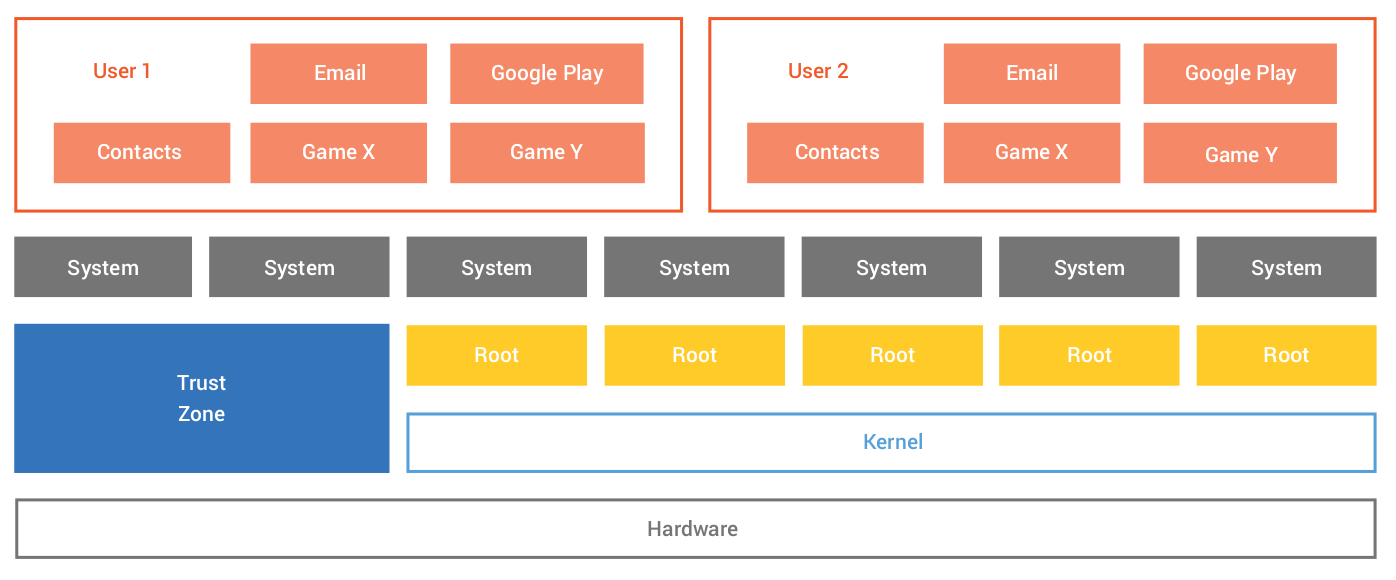
\includegraphics[width=\linewidth]{android_security_model}
	    \label{fig:ch01:sandbox}
    \end{subfigure}
    \caption{Aislamiento de las aplicaciones según su UID.}
 \end{figure}
\end{frame}
\begin{frame}
 \frametitle{Modelo de Android}
 \begin{small}
 \begin{itemize}
     \item Podemos clasificar los permisos según el riesgo implícito al otorgarlos:
     \begin{multicols}{2}
     \begin{itemize}[<+->]\small
      \item \emph{\textbf<5->{Normal}}
      \item \emph{\textbf<5->{Dangerous}}
      \item \emph{\invisible<5->{Signature}}
      \item \emph{\invisible<5->{Signature/System}}
     \end{itemize}
     \end{multicols}\pause
     \item A partir de la versión 6.0 se propone un nuevo modelo de permisos:\pause
         \begin{figure}[btp]
            \begin{subfigure}{0.4\linewidth}
            \centering
                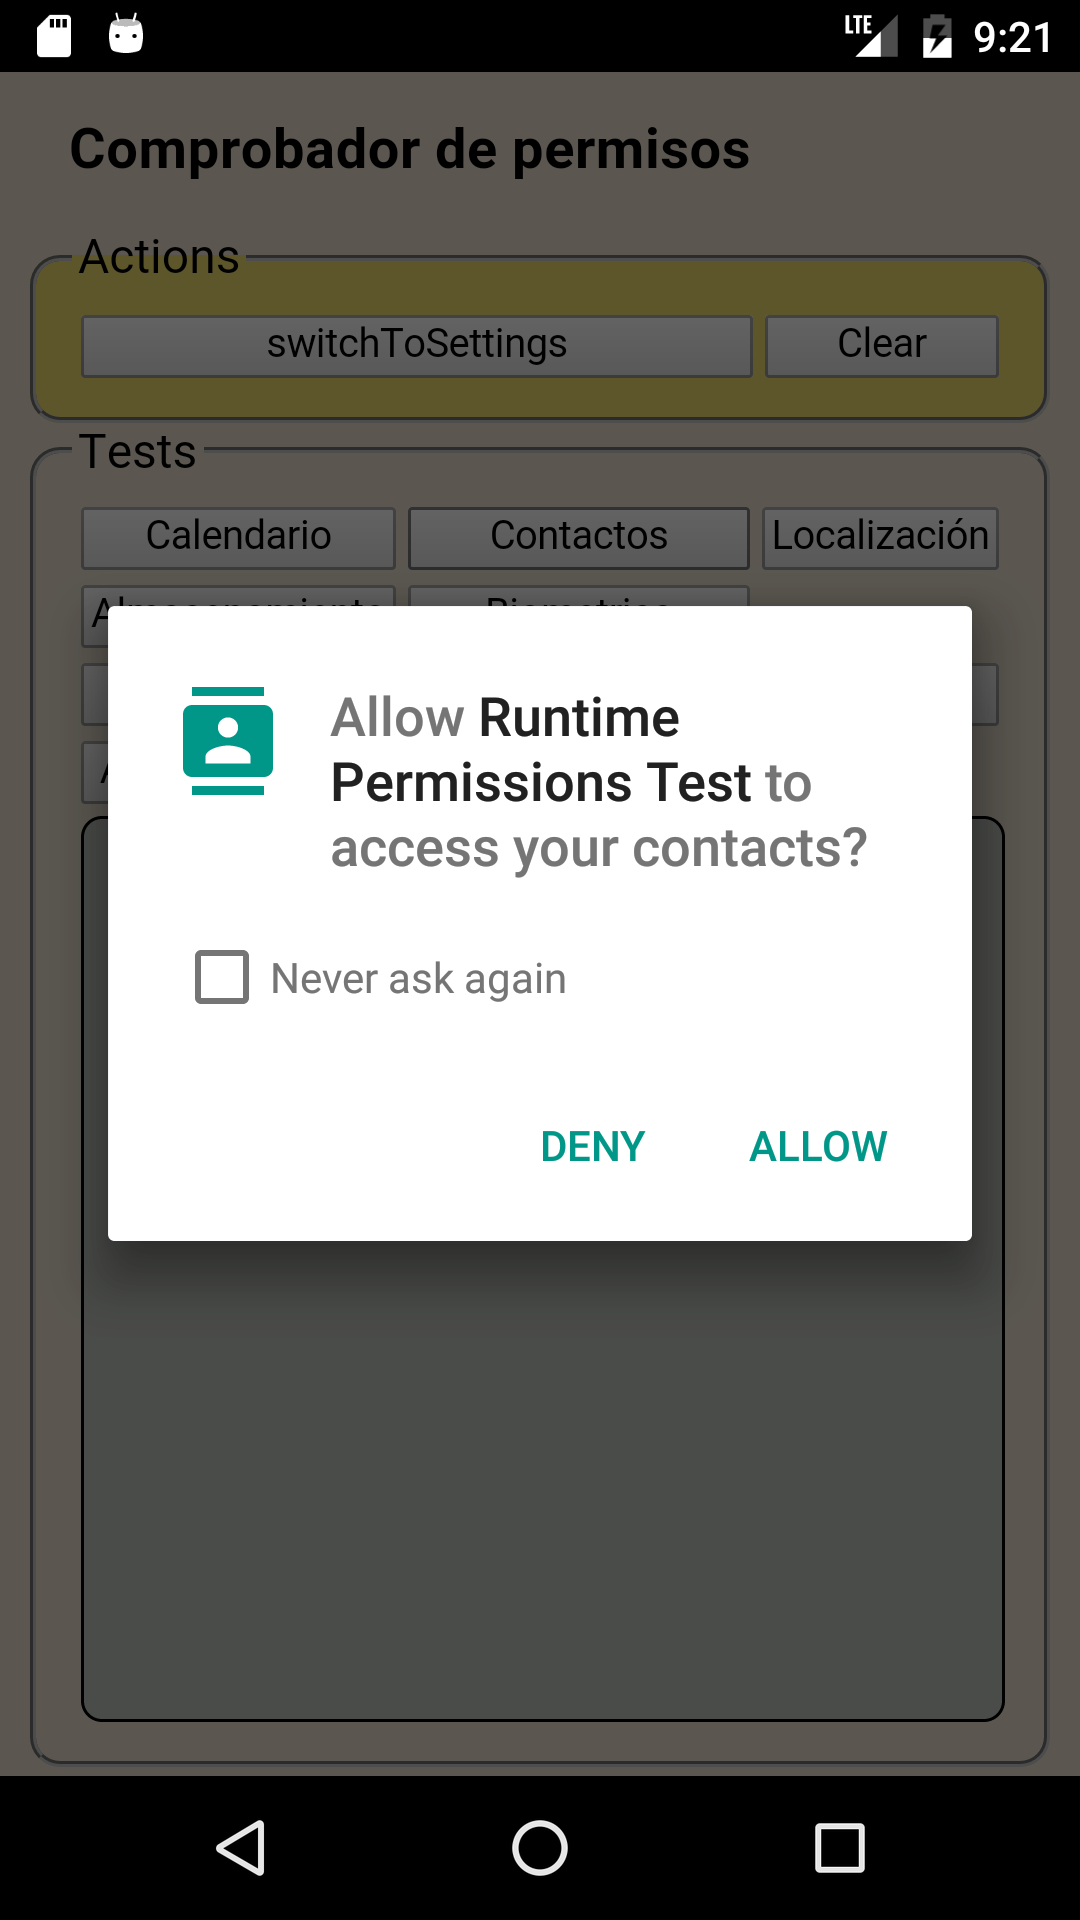
\includegraphics[width=.5\linewidth]{allow_contact}
                \caption{Solicitud de un permiso.}
            \end{subfigure}
        \begin{subfigure}{0.4\linewidth}\pause
        \centering
            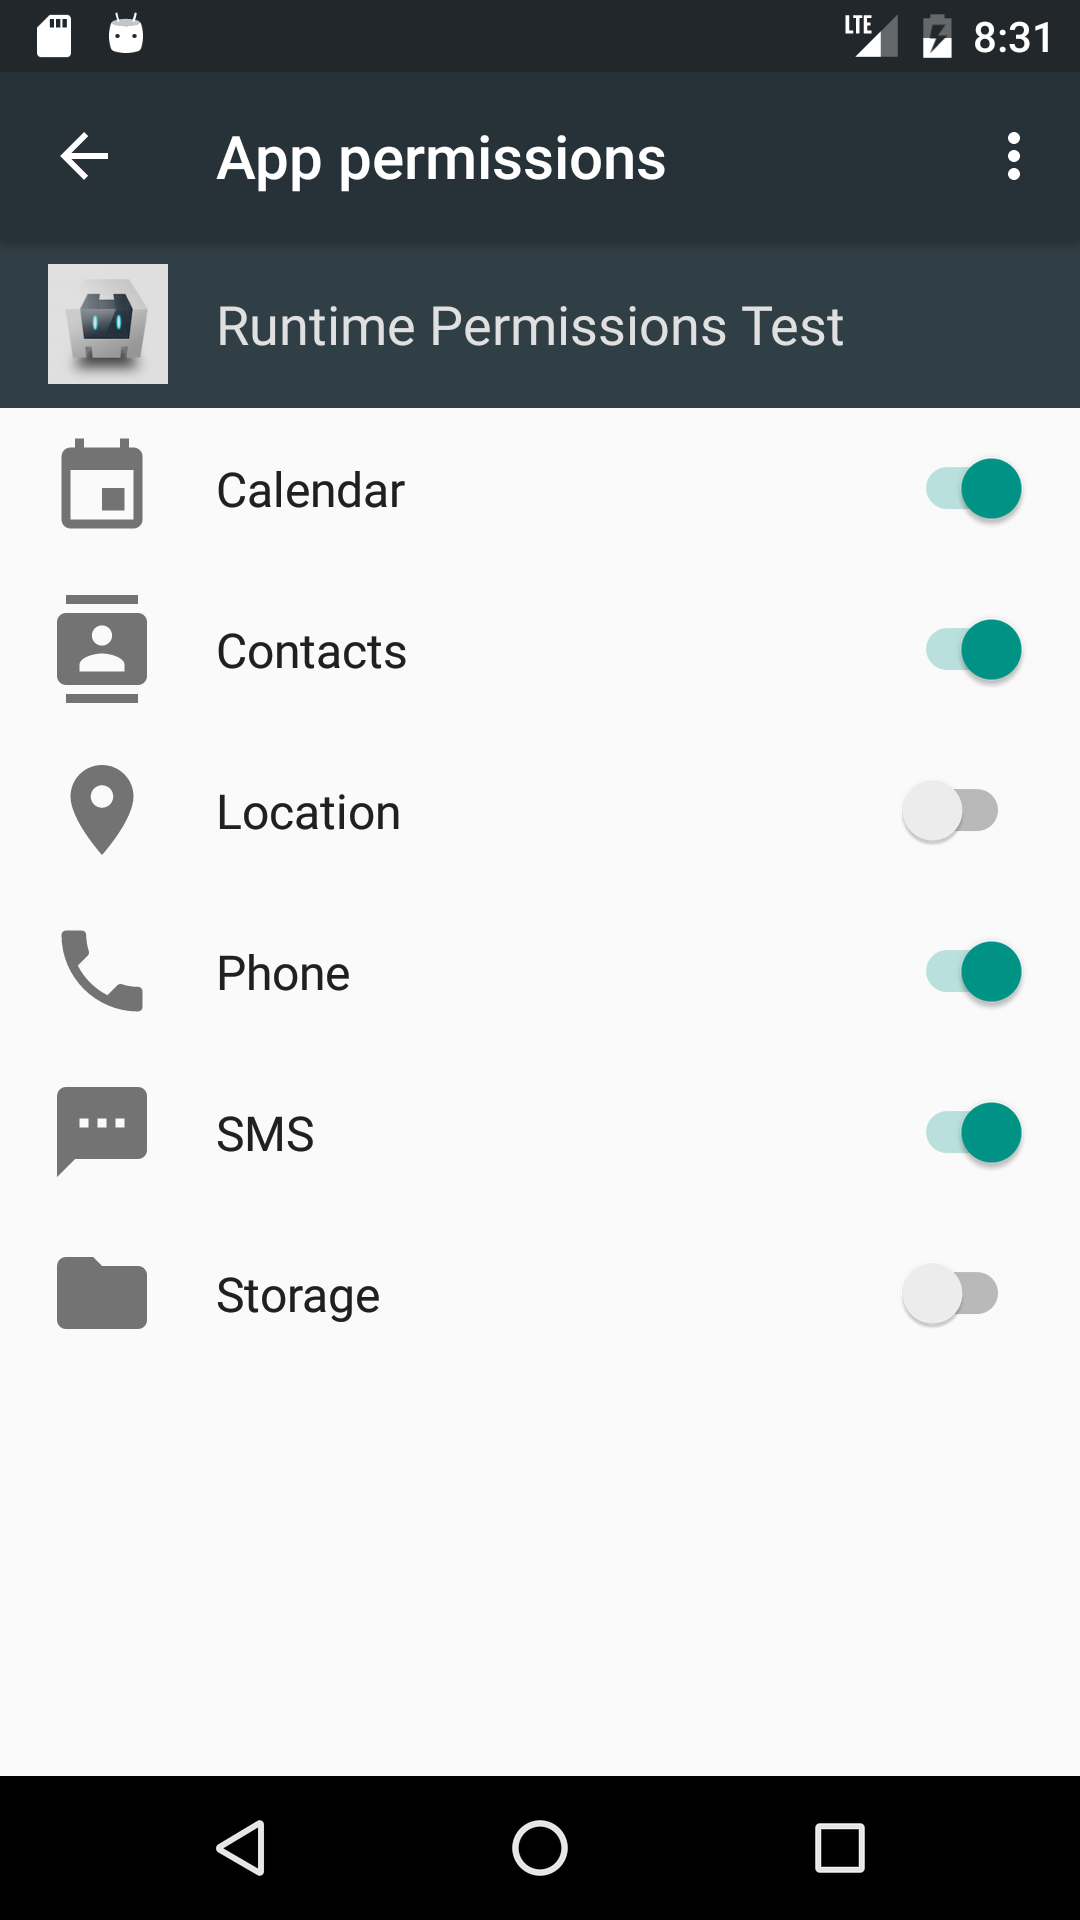
\includegraphics[width=.5\linewidth]{app-permissions}
            \caption{Listado de los permisos.}
    	\end{subfigure}
    	\caption{Nuevo modelo de permisos.}
        \end{figure}
 \end{itemize}
  \end{small}
\end{frame}


%\subsection{Modelo de iOS}
\begin{frame}
 \begin{center}
  \LARGE Modelo de iOS
 \end{center}
\end{frame}
\begin{frame}
 \frametitle{Modelo de iOS}
 \begin{figure}[tH]
  \begin{subfigure}{0.7\linewidth}
   \begin{itemize}
    \item iOS es un sistema operativo para dispositivos móviles de la multinacional Apple Inc. diseñado para ser
seguro. \pause
    \item Las principales características de seguridad no son configurables y vienen habilitadas por defecto.
   \end{itemize}
  \end{subfigure}
  \begin{subfigure}{0.25\linewidth}\pause
    \centering
    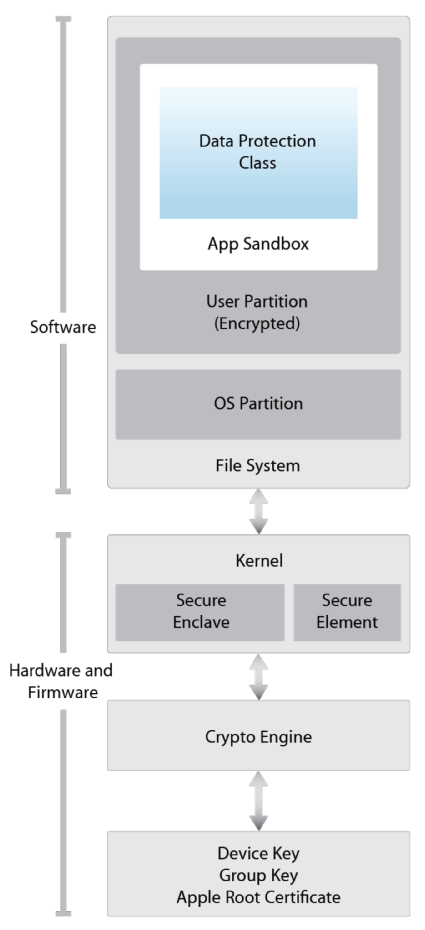
\includegraphics[width=\linewidth]{ios_security_architecture}
  \end{subfigure}
  \caption{Entorno seguro de iOS.}
\end{figure}
\end{frame}
\begin{frame}
 \frametitle{Modelo de iOS}
 \begin{itemize}
  \item Las aplicaciones pueden solicitar un permiso solamente mientras se esté ejecutando. \pause
 \end{itemize}
 \begin{figure}[hbtp]
    \centering
    \begin{subfigure}{0.49\linewidth}
    \centering
    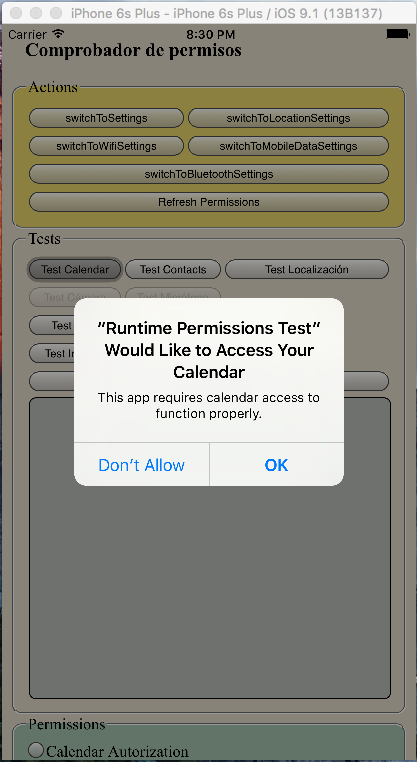
\includegraphics[width=.5\linewidth]{calendar_request_ios}
    \caption{Solicitud de un permiso.}
    \end{subfigure}
    \begin{subfigure}{0.49\linewidth}
    \centering
     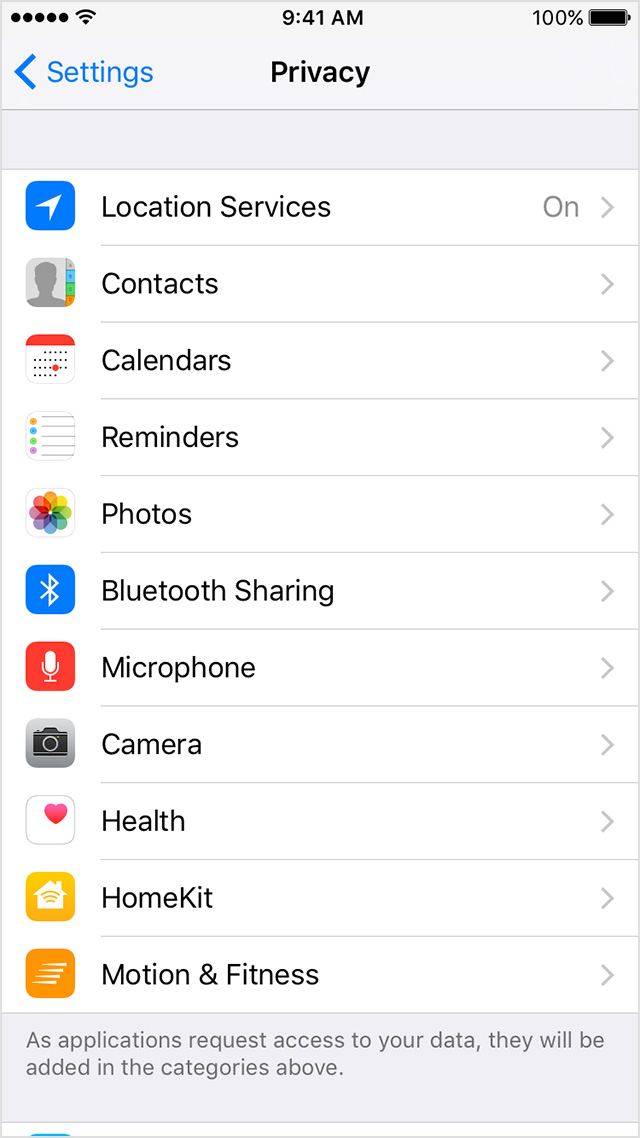
\includegraphics[width=.5\linewidth]{settings-privacy}
    \caption{Control de privacidad.}
    \end{subfigure}
    \caption{Sistema de permisos de iOS 9.}
 \end{figure}
\end{frame}
